\subsection{任务二}
本任务基于任务一计算得到的S盒线性近似表（LAT），搜索一条4轮迭代线性路线并计算其偏差。
% \begin{figure}[H]
%     \centering
%     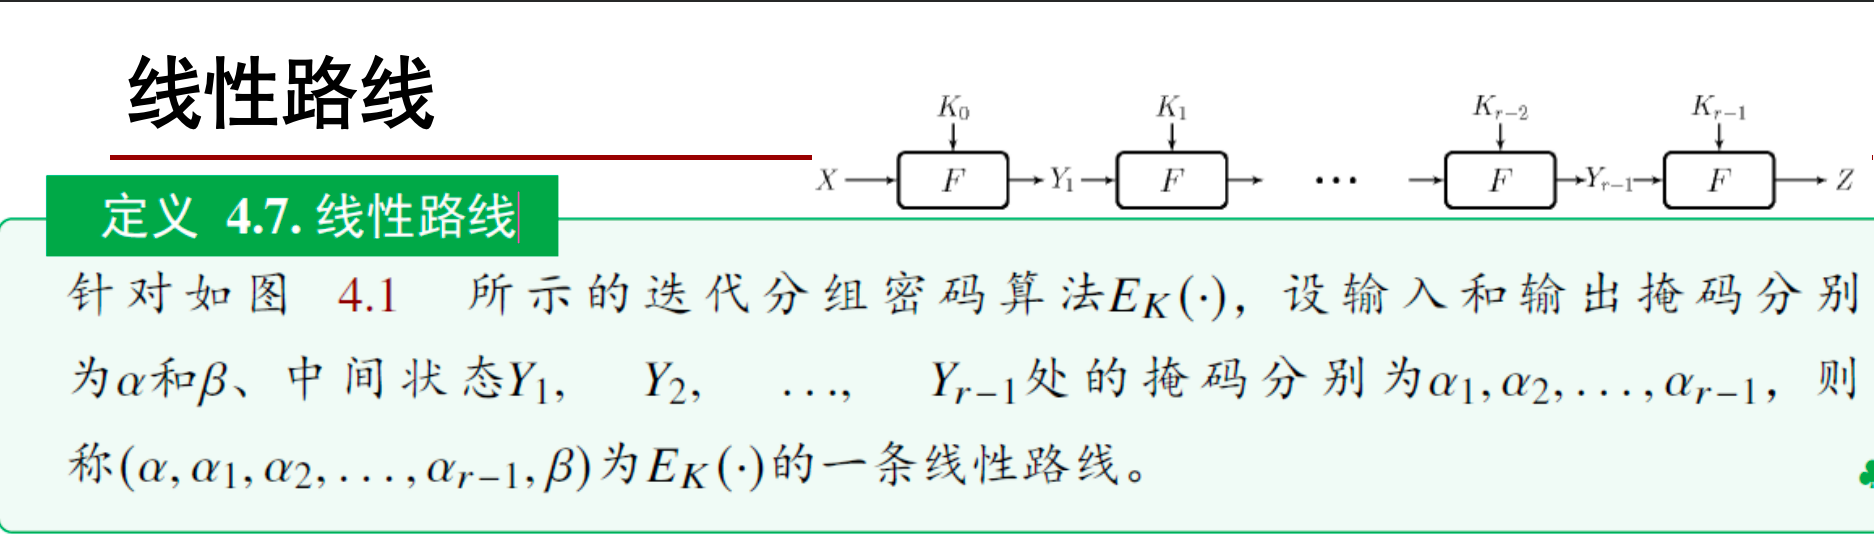
\includegraphics[width=0.95\textwidth]{figures/def1.png}
% \end{figure}
% 翻遍课本没找到迭代线性路线的定义，不过类比前面迭代差分路线，迭代的思路就是这一轮的输出要作为下一轮的输入，这样可以不断运作下去。所以输入掩码得和输出掩码一样，这样输出掩码又能作为下一轮的输入迭代下去，那4轮的迭代线性路线就是形如
% \[
% \alpha_1,\alpha_2,\alpha_3,\alpha_4,\alpha_1
% \]

\subsubsection{活跃S盒个数的考量}
% 那这还是一头雾水，主要是
CipherFour算法包含四个S盒，P置换使不同S盒的比特相互影响，增加了路线分析的复杂度。堆积引理和偏差分析建立在Markov假设之上，需要关注相关变量的独立性。因此，先考虑限制活跃S盒的数量，以简化分析，具体要求如图~\ref{fig:request}所示。
\begin{figure}[H]
    \centering
    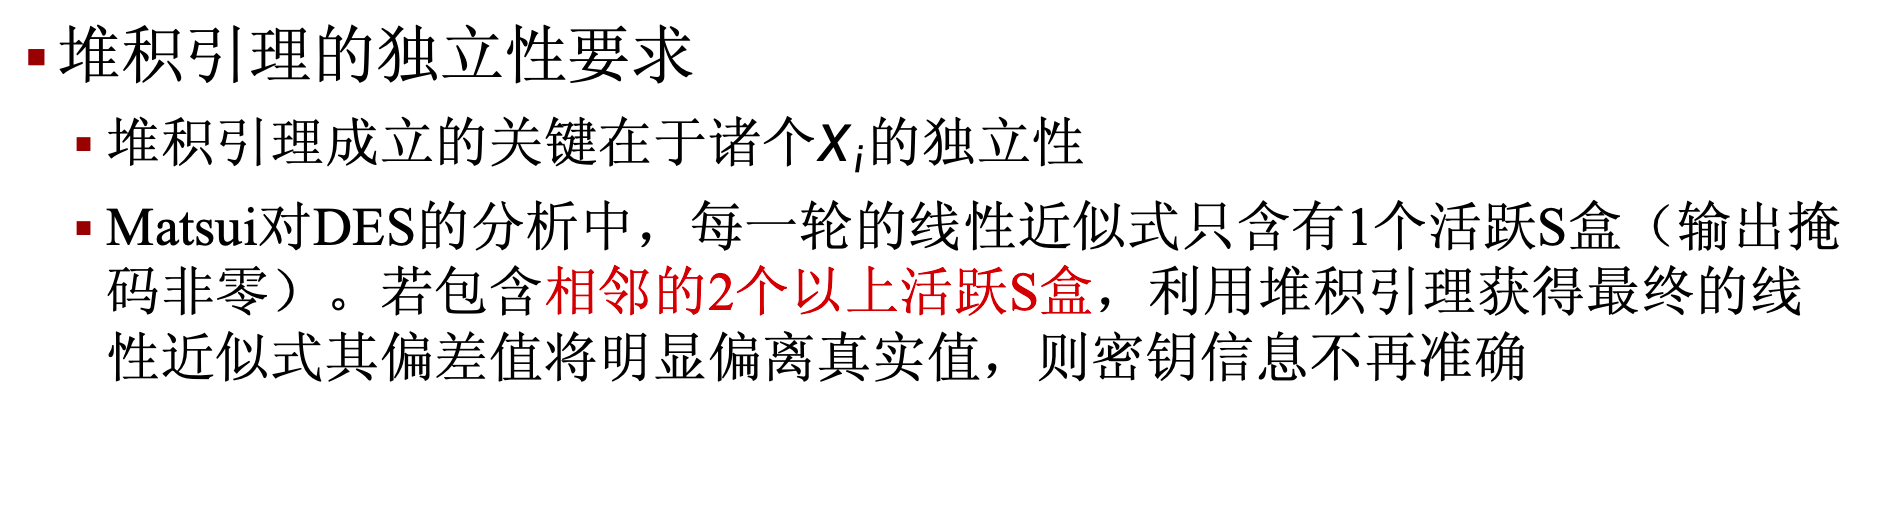
\includegraphics[width=0.95\textwidth]{figures/limit.png}
    \caption{堆积引理要求}
    \label{fig:request}
\end{figure}
采用相关度表示时，堆积引理的形式更为简洁。考虑输入掩码$\alpha=(\alpha_0,\alpha_1,\alpha_2,\alpha_3)$和输出掩码$\beta=(\beta_0,\beta_1,\beta_2,\beta_3)$，4个S盒对应的一轮S层相关度为
\[
c(\alpha,\beta)
=\prod_{j=0}^{3}c(\alpha_j,\beta_j)
\]
相关度为偏差的2倍，相关度较大的路线更有利于线性分析。由于\(c(0,0) = 1\)，可以优先考虑活跃S盒较少的路线。不过，为避免全零掩码对应的平凡情况，路线中至少需要一个活跃S盒。

不过，除$c(0,0) = 1$外，还需要考虑LAT中的其他掩码组合。前面的LAT中，除了(0,0)对应的表项为8外，任务一还找到了$B \rightarrow 3$这一组合，如下图所示。
\begin{figure}[H]
    \centering
    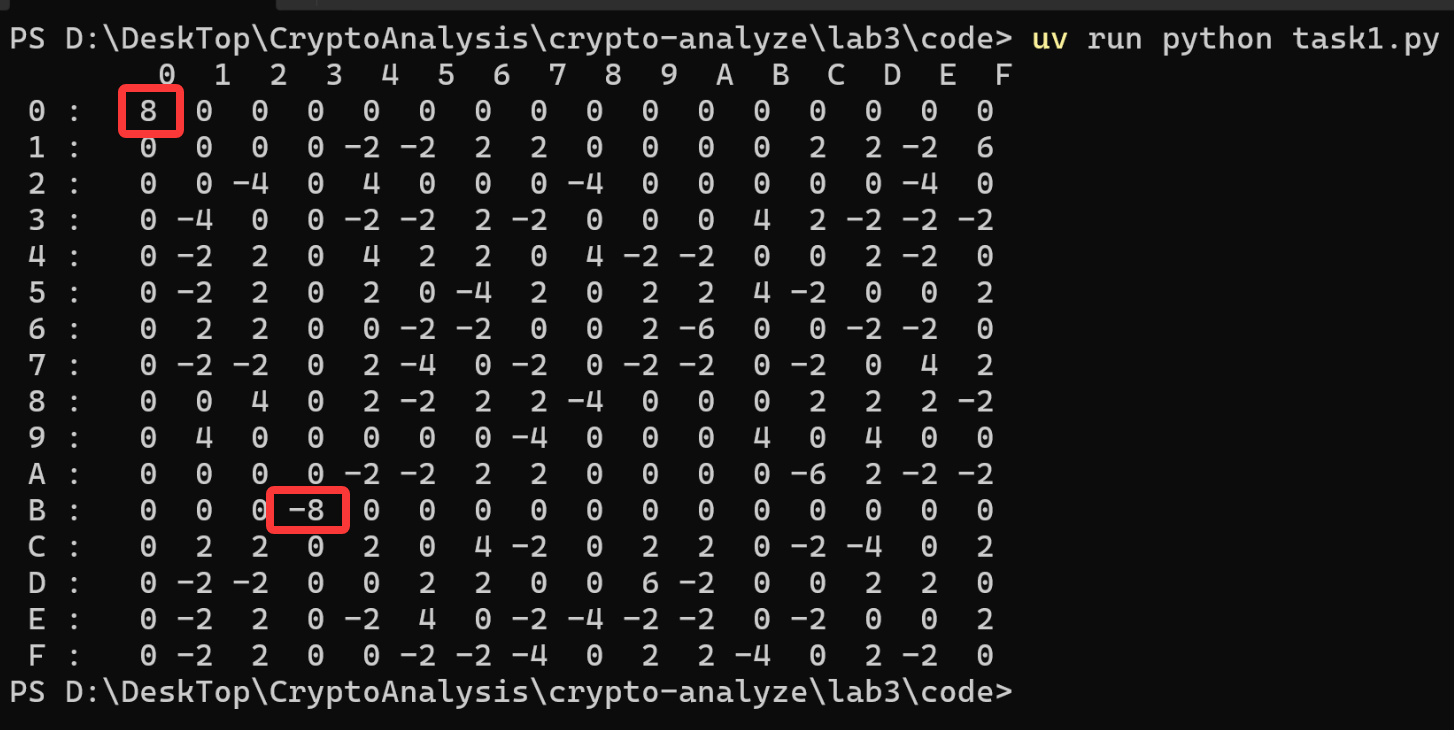
\includegraphics[width=0.95\textwidth]{figures/find1.png}
    \caption{LAT}
\end{figure}
也就是说$c(B,3) = 1$，从相关度看，该组合与(0,0)具有相同的效果，理论上也可以选用。但本实验还包含P层置换，引入该组合会增加后续分析的复杂度。为便于人工分析，先采用较简单的路线，选择(0,0)作为非活跃S盒的掩码，从仅有一个活跃S盒的情形开始讨论。

\subsubsection{贪心搜索思路}

与差分路线分析相比，线性路线分析还需要考虑线性变换对掩码的影响，如下图所示。
\begin{figure}[H]
    \centering
    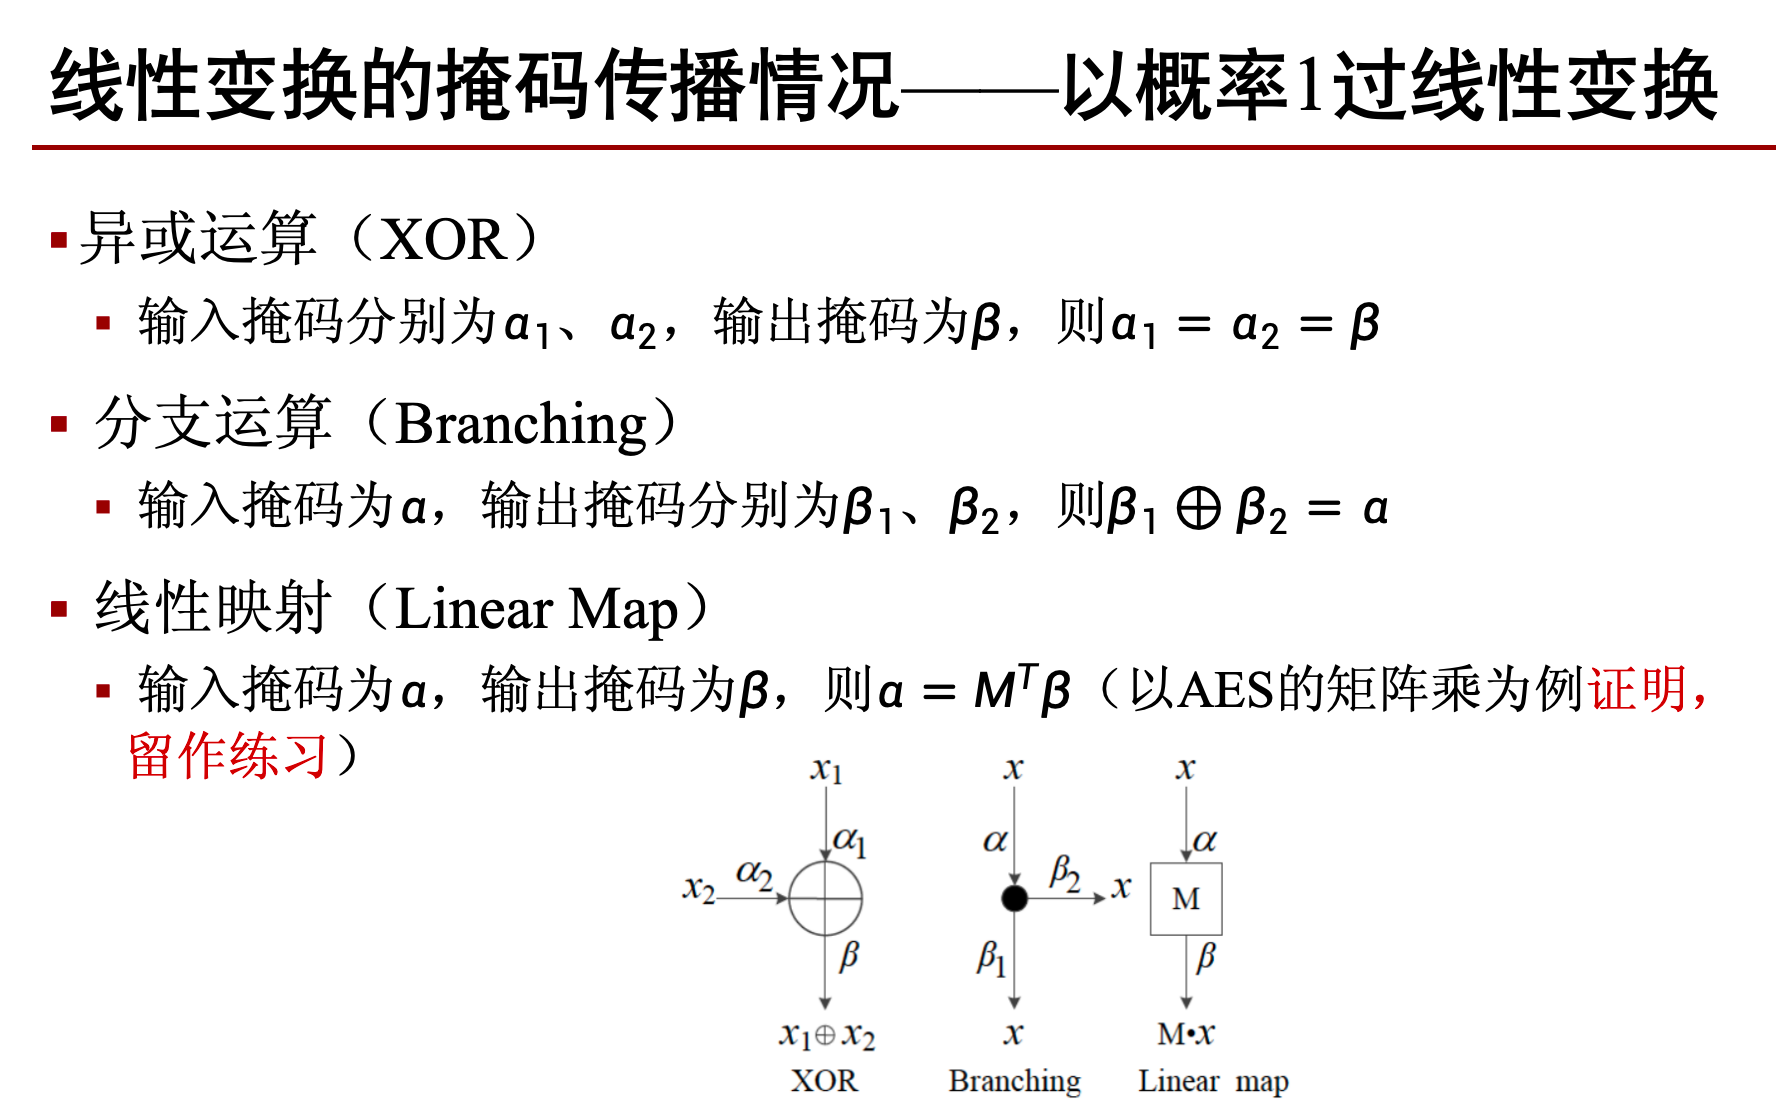
\includegraphics[width=0.95\textwidth]{figures/find2.png}
\end{figure}
线性掩码需要经过P置换。将该置换表示为矩阵，并仍记作P，可按下图的方法构造该矩阵。
\begin{figure}[H]
    \centering
    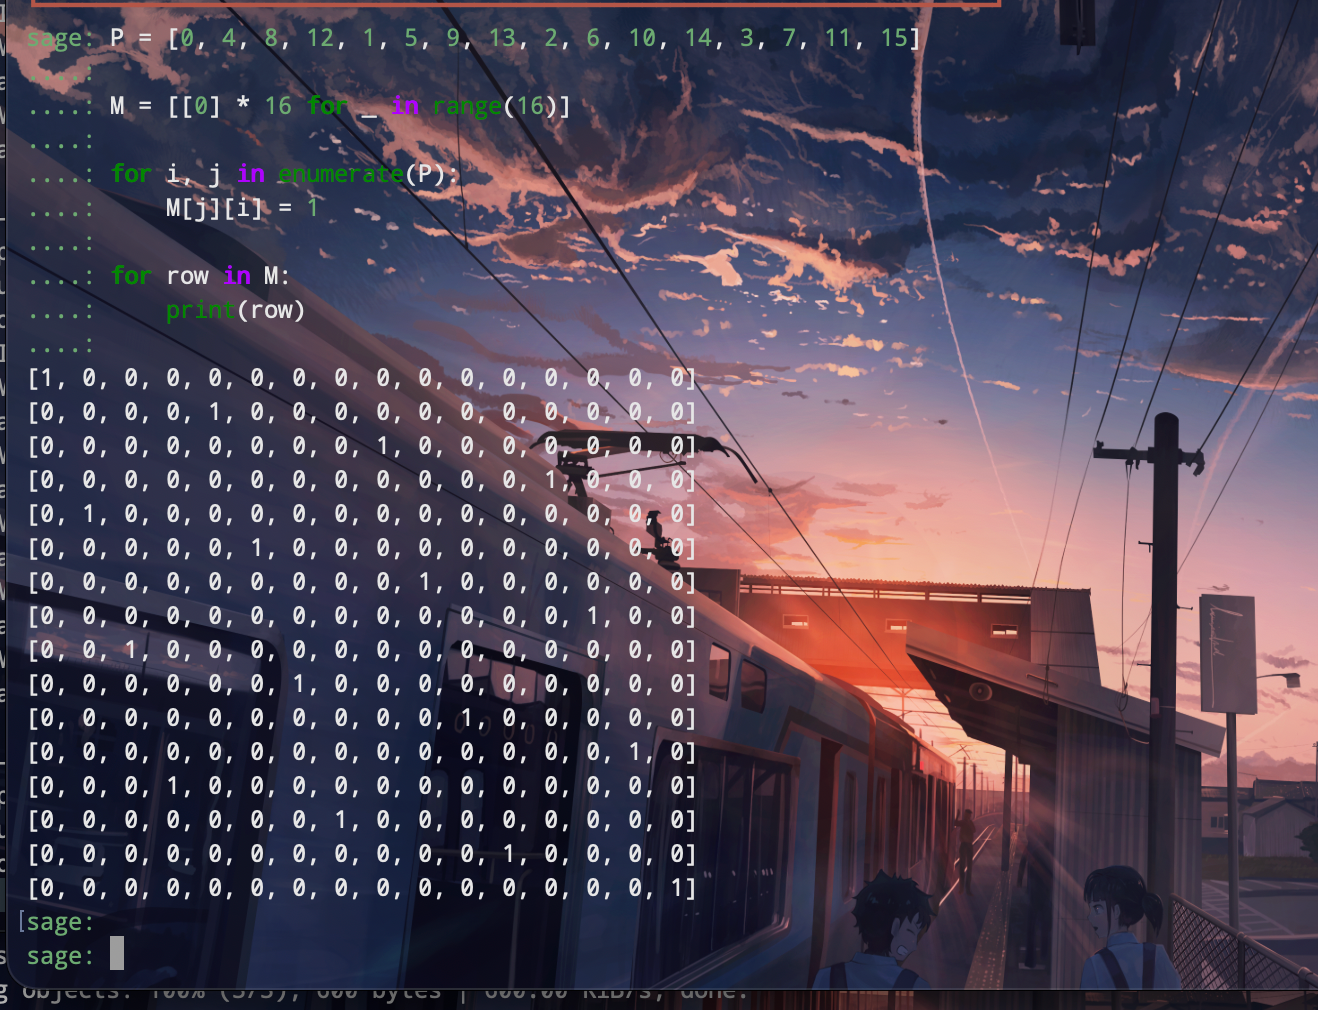
\includegraphics[width=0.95\textwidth]{figures/P.png}
\end{figure}
设第一轮的输入掩码为\(\alpha_1\)，输出掩码为\(\beta_1\)。若不考虑P置换，应满足$\beta_1 = \alpha_2$；引入P置换后，则应满足$\alpha_2 = P\beta_1$。为明确掩码的传播过程，先考虑如下初始状态：
\[(\alpha_{11},0,0,0) \xrightarrow{S} (\beta_{11},0,0,0)\xrightarrow{P} (\alpha_{21},\alpha_{22},\alpha_{23},\alpha_{24})\]
进一步得到如下四轮传播路线：
\[\alpha_1\xrightarrow{S}\beta_1\xrightarrow{P}
\alpha_2\xrightarrow{S}\beta_2\xrightarrow{P}
\alpha_3\xrightarrow{S}\beta_3\xrightarrow{P}
\alpha_4\xrightarrow{S}\beta_4\xrightarrow{P}
\alpha_1\]

为形成可执行的搜索算法，需要明确每一步的输出选择。P层的矩阵运算已经确定，而S层存在多个候选输出。以偏差尽可能大为目标，可以在候选中选择偏差最大的输出，这对应于一种贪心搜索思路。由于本任务只要求找到一条满足条件的路线，可以先采用这一方法。虽然贪心算法不保证全局最优，但可以从局部较优的选择出发，寻找满足要求的路线。

为进一步简化P置换带来的影响，可以先寻找该置换的不动点，即令$P\beta = \beta$，等价于$(P-I)\beta = 0$。若该矩阵不满秩，则存在非零解。观察前面的矩阵可知，P的第一行第一列为1，减去单位矩阵后，第一行全为0，因此该矩阵不满秩。由此可以选择满足上述条件的$\beta$，如下图所示。
\begin{figure}[H]
    \centering
    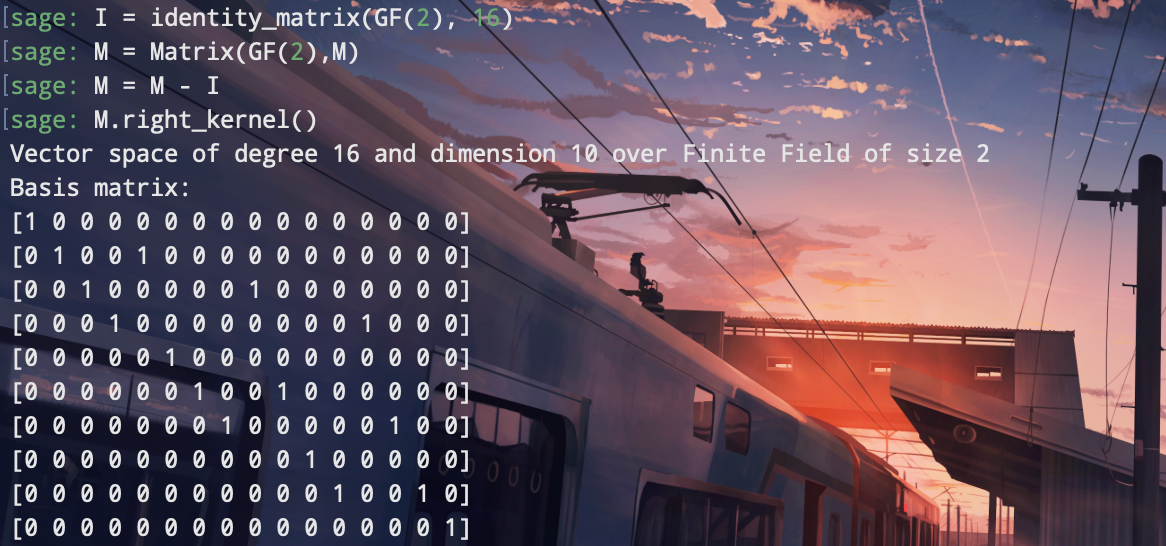
\includegraphics[width=0.95\textwidth]{figures/solution.png}
\end{figure}
例如，$\beta = 1000000000000000$，也就是\(\beta = (8,0,0,0)\)。进一步考虑迭代性质，可以先寻找一轮即可闭合的路线，再将其重复4次，从而避免直接搜索完整的四轮路线，即
\[\alpha_1\xrightarrow{S}\beta_1\xrightarrow{P} \alpha_1\]
还可以放宽$P\beta = \beta$这一限制，直接要求\[P(\beta_1) = \alpha_1\]

\subsubsection{单轮迭代路线的搜索与结果}

在上述约束下，$\beta_1$可直接由$\alpha_1$确定，从而简化搜索算法。此前限制活跃S盒的数量主要是为了方便计算；在仅搜索单轮迭代路线时，可以重新考虑这一限制。虽然可以从一个、两个活跃S盒的情形依次尝试，但全部非零输入掩码仅有$2^{16}-1$种，因此可直接遍历全部$2^{16}-1$个非零\(\alpha\)，覆盖不同活跃S盒数量的情况。随后通过\(P^{-1}\)计算\(\beta\)，查询LAT并将各S盒的相关度相乘，选择绝对相关度最大的候选，再将该路线重复四轮。对应伪代码如算法~\ref{alg:task2-trail}所示。

\begin{algorithm}[H]
    \caption{CipherFour四轮迭代线性路线的搜索}
    \label{alg:task2-trail}
    \begin{algorithmic}[1]
        \Require 4比特S盒线性近似表$\mathrm{LAT}[0..15,0..15]$，16比特置换$P$
        \Ensure 四轮迭代线性路线及其理论偏差
        \State $\alpha^*\gets 0,\ \beta^*\gets 0,\ C^*\gets 0$
        \For{$\alpha=1,\ldots,2^{16}-1$}
            \State $\beta\gets P^{-1}(\alpha)$
            \State $C\gets 1$
            \For{$j=0,\ldots,3$}
                \State $a\gets(\alpha\gg 4j)\& 0xF$
                \State $b\gets(\beta\gg 4j)\& 0xF$
                \State $C\gets C\cdot\mathrm{LAT}[a,b]/8$
            \EndFor
            \If{$|C|>|C^*|$ \textbf{or} $(|C|=|C^*|\ \textbf{and}\ \alpha>\alpha^*)$}
                \State $\alpha^*\gets\alpha$
                \State $\beta^*\gets\beta$
                \State $C^*\gets C$
            \EndIf
        \EndFor
        \State $C_4\gets (C^*)^4$
        \State $\varepsilon_4\gets C_4/2$
        \State $T\gets[\alpha^*,\alpha^*,\alpha^*,\alpha^*,\alpha^*]$
        \State \Return $T,\beta^*,\varepsilon_4$
    \end{algorithmic}
\end{algorithm}

代码运行结果如图~\ref{fig:task2-trail}所示。
\begin{figure}[H]
    \centering
    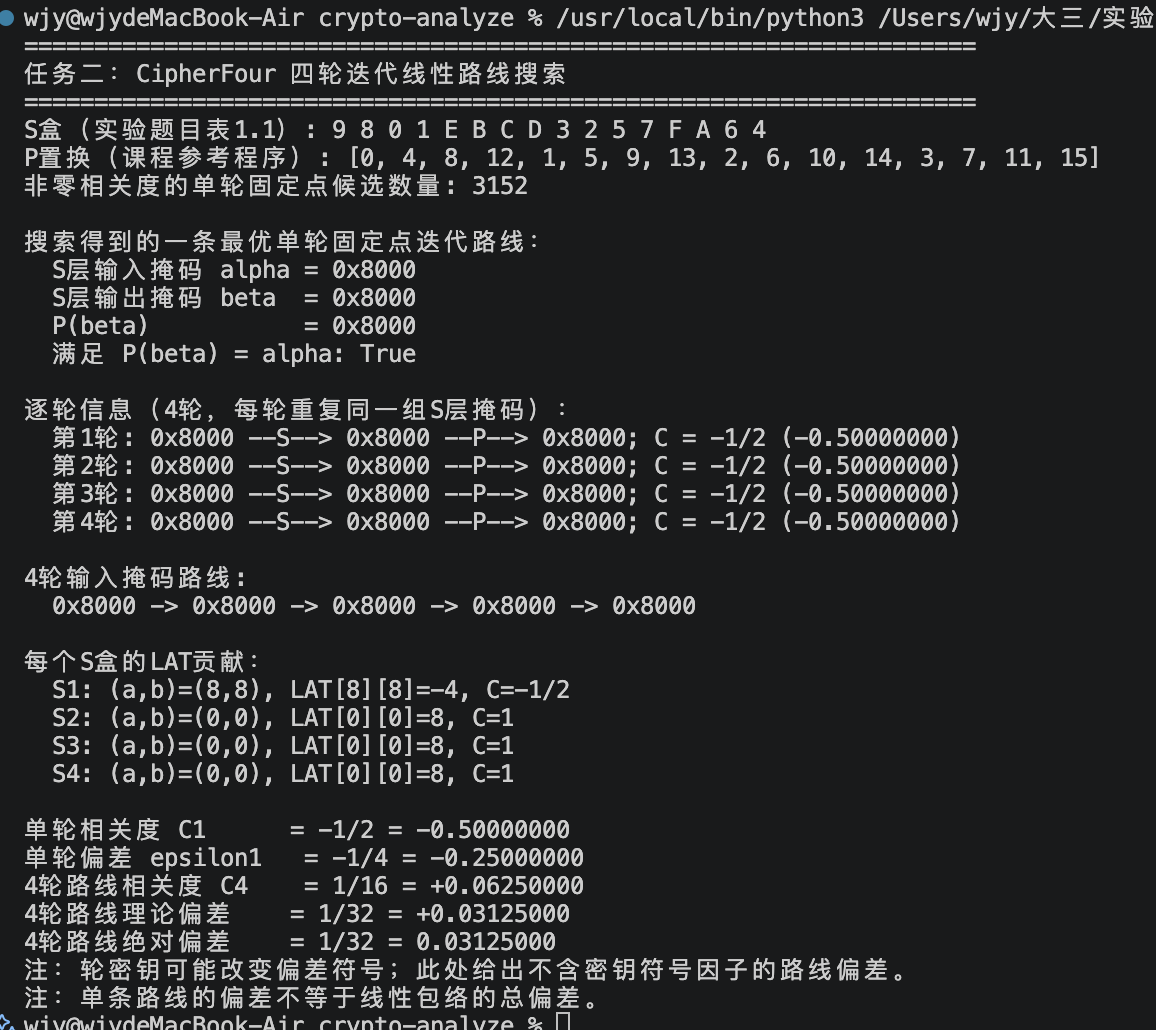
\includegraphics[width=0.95\textwidth]{figures/task2.png}
    \caption{任务二四轮迭代线性路线搜索结果}
    \label{fig:task2-trail}
\end{figure}
程序共找到$3152$个单轮相关度非零的候选，其中一条绝对相关度最大的路线满足
\[
\alpha=0x8000,\qquad
\beta=0x8000,\qquad
P(0x8000)=0x8000.
\]
因此，该路线可迭代4轮，得到
\[
0x8000\longrightarrow0x8000\longrightarrow0x8000
\longrightarrow0x8000\longrightarrow0x8000.
\]
对于每一轮，仅第一个S盒的输入、输出掩码非零，分别为$(8,8)$；其余3个S盒的掩码均为$(0,0)$。由任务一所得LAT可知
\[
\mathrm{LAT}[8,8]=-4,\qquad
\mathrm{LAT}[0,0]=8.
\]
故单轮相关度为
\[
C_1
=\frac{-4}{8}\left(\frac{8}{8}\right)^3
=-\frac12,
\]
相应的单轮偏差为$\varepsilon_1=C_1/2=-1/4$。根据堆积引理（Piling-up Lemma），4轮\textbf{单条线性路线}的相关度为
\[
C_4=\prod_{i=1}^{4}C_i
=\left(-\frac12\right)^4
=\frac1{16}.
\]
从而得到不计密钥常数项时的理论偏差
\[
\varepsilon_4=\frac{C_4}{2}=\frac1{32}=0.03125.
\]
上述结果来自单轮路线重复四次的搜索，仍需进一步判断其是否为全部四轮迭代路线中的最优解。例如，还可以考虑将两条两轮路线拼接，或直接构造一条四轮闭合路线。搜索这些路线时，活跃S盒的数量再次影响分析规模，因为中间状态无法像单轮情形一样由P置换直接确定。针对这一问题，我们借助AI进行进一步分析，结果如下。
\begin{figure}[H]
    \centering
    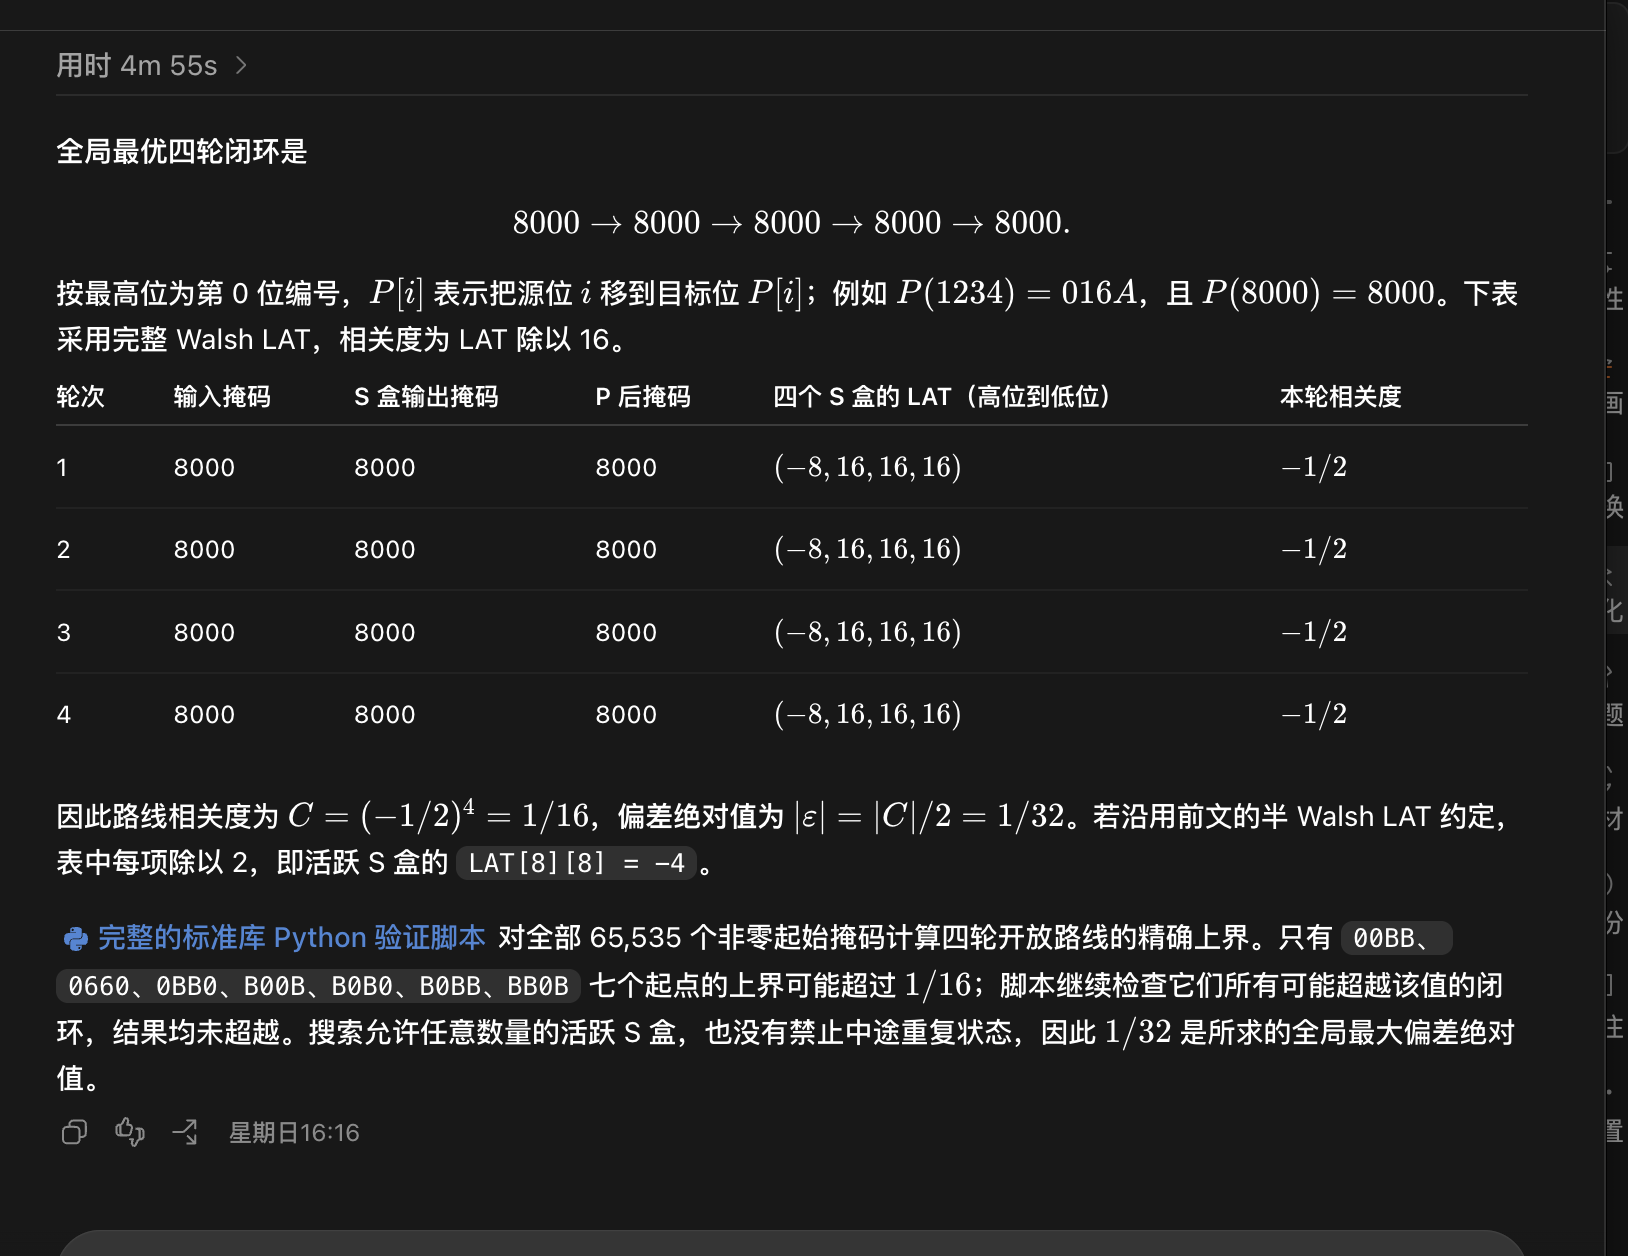
\includegraphics[width=0.95\textwidth]{figures/find3.png}
\end{figure}
该辅助分析给出的全局最优路线与本实验搜索所得路线一致。
